\documentclass{beamer}
\usepackage{graphicx}
\usepackage{xcolor}
\usepackage{tikz}

% 自定义颜色
\definecolor{purpleblue}{RGB}{80, 80, 180}
\definecolor{lightgray}{RGB}{230, 230, 230}
\definecolor{novelPurple}{RGB}{98, 54, 255} 
\definecolor{darkgray}{RGB}{50, 50, 50}

% 主题设置
\usetheme{Madrid}  
\usecolortheme{dolphin} 

% 设置字体（移除 fontspec，确保 pdfLaTeX 兼容）
\setbeamerfont{title}{size=\Large,series=\bfseries}
\setbeamerfont{frametitle}{size=\LARGE,series=\bfseries}
\setbeamercolor{frametitle}{fg=white, bg=novelPurple}
\setbeamercolor{title}{fg=white, bg=purpleblue}

% 封面信息
\title[SAT Unit 2.3.1 ]{\textbf{SAT Unit 2.3.1\\ Polynomial and Rational Function}}
\author{\textbf{Jack Zeng}}
\institute{\textcolor{white}{\textbf{Novel Prep}}}
\date{\today} 

\begin{document}

% --- Title Slide ---
\begin{frame}
    \titlepage
    \vfill
    \begin{flushright}
        \textcolor{purpleblue}{\Huge \textbf{Novel Prep}}
    \end{flushright}
\end{frame}


\begin{frame}
    \begin{tikzpicture}[remember picture, overlay]

        \shade[top color=softPurple, bottom color=softGray] 
            (current page.north west) rectangle (current page.south east);

        \fill[white, opacity=0.3] (current page.center) circle (4cm);
        

        \node[align=center] at (current page.center) {
            {\Huge\bfseries\textcolor{purpleblue}{Novel Prep}} \\[0.5cm]
            {\Large\itshape\textcolor{lightText}{Excellence in SAT Prep}}
        };
        \foreach \x in {1,2,3,4,5} {
            \fill[purpleblue, opacity=0.2] (rand*10-5, rand*7-3.5) circle (0.1+\x*0.05);
        }
        ;
    \end{tikzpicture}
\end{frame}






\begin{frame}{Overview}
    \tableofcontents
\end{frame}

\begin{frame}
\section{Polynomial Functions}
    \begin{tikzpicture}[remember picture, overlay]

        \shade[top color=softPurple, bottom color=softGray] 
            (current page.north west) rectangle (current page.south east);

        \fill[white, opacity=0.3] (current page.center) circle (4cm);
        

        \node[align=center] at (current page.center) {
            {\LARGE\bfseries\textcolor{purpleblue}{Polynomial Function}} \\[0.5cm]
            {\Large\itshape\textcolor{lightText}{Excellence in SAT Prep}}
        };
        \foreach \x in {1,2,3,4,5} {
            \fill[purpleblue, opacity=0.2] (rand*10-5, rand*7-3.5) circle (0.1+\x*0.05);
        }
        ;
    \end{tikzpicture}
\end{frame}

% --- Add this after the second title slide ---





\begin{frame}{Definition of Polynomial Functions}
\small

\textbf{Definition of Polynomial:}

An expression of the form:
\[
a_nx^n + a_{n-1}x^{n-1} + \cdots + a_1x + a_0
\]
where:
\begin{itemize}
    \item $n$ is a nonnegative integer (called the \textbf{degree}).
    \item $a_n, a_{n-1}, \ldots, a_0$ are real numbers (called \textbf{coefficients}).
\end{itemize}

\vspace{0.3cm}
\textbf{Terminology:}
\begin{itemize}
    \item \textbf{Monomial:} A polynomial with one term (e.g., $5x^3$)
    \item \textbf{Binomial:} Two unlike terms (e.g., $x^2 + 3x$)
    \item \textbf{Trinomial:} Three unlike terms (e.g., $x^2 + 3x + 2$)
    \item \textbf{Like Terms:} Terms that have the same variable and exponent (e.g., $3x^2$ and $-2x^2$)
\end{itemize}



\end{frame}

\begin{frame}{Structure and Degree of Polynomials}
\small

\textbf{Degree:}
\begin{itemize}
    \item The \textbf{degree of a monomial} is the sum of the exponents of all variables in that term.
    \item The \textbf{degree of a polynomial} is the greatest degree among all its terms.
\end{itemize}

\vspace{0.3cm}
\textbf{Components of a Polynomial:}
\begin{itemize}
    \item \textbf{Leading Term:} The term with the highest degree.
    \item \textbf{Leading Coefficient:} The coefficient of the leading term.
    \item \textbf{Constant Term:} A term with no variable (degree 0).
\end{itemize}

\vspace{0.3cm}
\textbf{Example:}
\[
f(x) = 3x^3 - 4x^2 + 7x + 18
\]
\begin{itemize}
    \item Degree: 3 \quad Leading Coefficient: 3 \quad Constant: 18
\end{itemize}

\end{frame}


\begin{frame}{Zeros of Polynomial Functions and Graph Behavior}
\begin{columns}

% Left column: Definitions and properties
\begin{column}{0.58\textwidth}
\small
\textbf{Real Zeros of Polynomial Functions}

When $f$ is a polynomial function and $a$ is a real number, the following are equivalent:
\begin{enumerate}
    \item $x = a$ is a \textbf{zero} of $f$.
    \item $x = a$ is a \textbf{solution} of $f(x) = 0$.
    \item $(x - a)$ is a \textbf{factor} of $f(x)$.
    \item $(a, 0)$ is an \textbf{$x$-intercept} of the graph of $f$.
\end{enumerate}

\vspace{0.1cm}
\textbf{Repeated Zeros and Multiplicity}
\begin{itemize}
    \item A factor $(x - a)^k$, $k > 1$, yields a \textbf{repeated zero} $x = a$ of \textbf{multiplicity} $k$:
    \begin{itemize}
        \item If $k$ is odd: the graph \textbf{crosses} the $x$-axis.
        \item If $k$ is even: the graph \textbf{touches} the $x$-axis.
    \end{itemize}
\end{itemize}
\end{column}

% Right column: Graph image
\begin{column}{0.35\textwidth}
    \centering
    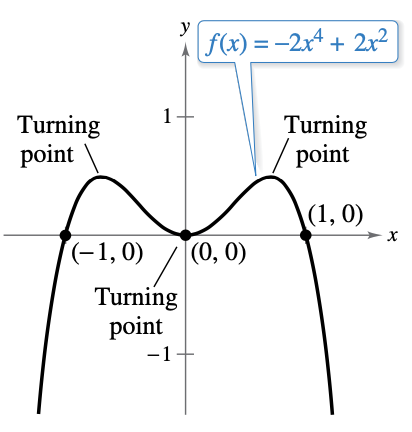
\includegraphics[width=\linewidth]{E26.png}
    \vspace{0.2cm}

\end{column}

\end{columns}
\end{frame}
\begin{frame}{Question: Polynomial Matches the Graph}
\small

\textbf{The graph of a function $f$ is shown. Which of the following functions could define $f$?}

\begin{center}
    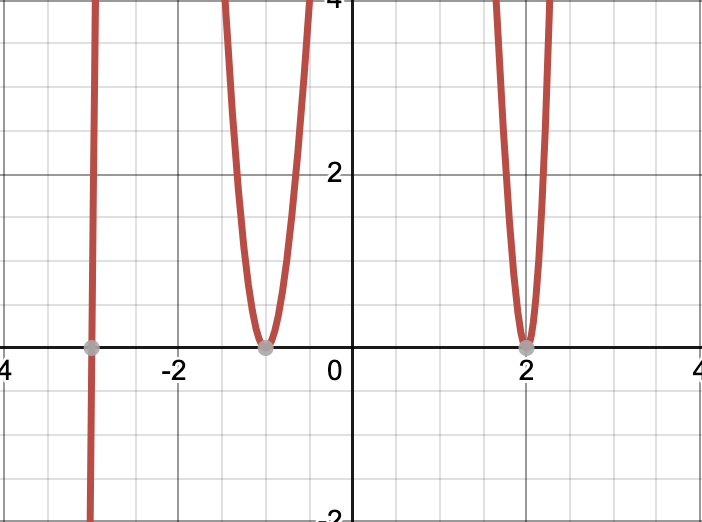
\includegraphics[width=0.40\linewidth]{E27.png} % Replace with your image filename
\end{center}

\vspace{0.2cm}
\textbf{Choices:}
\begin{enumerate}
    \item[\textbf{A.}] $f(x) = (x - 3)(x - 1)^2(x + 2)^2$
    \item[\textbf{B.}] $f(x) = (x - 3)^2(x - 1)(x + 2)$
    \item[\textbf{C.}] $f(x) = (x + 3)(x + 1)^2(x - 2)^2$
    \item[\textbf{D.}] $f(x) = (x + 3)^2(x + 1)(x - 2)$
\end{enumerate}

\end{frame}



\begin{frame}{Answer: Identifying a Polynomial from Its Graph}
\small

\textbf{Goal:} Match the graph of $f(x)$ to one of the given polynomial equations.

\vspace{0.2cm}
\textbf{Step 1: Identify the Zeros}
\begin{itemize}
    \item The graph crosses/touches the $x$-axis at:
    \[
    x = -3,\quad x = -1,\quad x = 2
    \]
\end{itemize}

\vspace{0.2cm}
\textbf{Step 2: Analyze Multiplicities}
\begin{itemize}
    \item Touches at $x = -1$ and $x = 2$ $\Rightarrow$ even multiplicity (likely squared).
    \item Crosses at $x = -3$ $\Rightarrow$ odd multiplicity (likely linear).
\end{itemize}

\vspace{0.2cm}
\textbf{Step 3: Determine Equation}
\[
f(x) = (x + 3)(x + 1)^2(x - 2)^2
\]

\vspace{0.2cm}
\textbf{Correct Answer:} \textcolor{blue}{C}
\end{frame}




\begin{frame}{\textbf{Question: Solving a Factored Equation with Radicals}}
\[
\frac{5}{8}(5x + 8)\left(x + \sqrt{5k + 8}\right)\left(x - \sqrt{5k + 8}\right) = 0
\]

In the given equation, $k$ is a positive constant. The product of the solutions to the equation is $64$. What is the value of $k$?
\end{frame}


\begin{frame}{\textbf{Answer and Explanation}}
We are given:
\[
\frac{5}{8}(5x + 8)(x + \sqrt{5k + 8})(x - \sqrt{5k + 8}) = 0
\]

The three roots come from:
\begin{itemize}
    \item $5x + 8 = 0 \Rightarrow x = -\frac{8}{5}$
    \item $x + \sqrt{5k + 8} = 0 \Rightarrow x = -\sqrt{5k + 8}$
    \item $x - \sqrt{5k + 8} = 0 \Rightarrow x = \sqrt{5k + 8}$
\end{itemize}

So the roots are:
\[
x = -\frac{8}{5},\quad -\sqrt{5k + 8},\quad \sqrt{5k + 8}
\]

Let’s compute the product of the roots (since the coefficient $\frac{5}{8}$ does not affect the roots):
\[
\left(-\frac{8}{5}\right) \cdot \left(-\sqrt{5k + 8}\right) \cdot \left(\sqrt{5k + 8}\right) = \frac{8}{5}(5k + 8)
\]


\end{frame}
\begin{frame}{Answer and Explanation}
We're told the product of the solutions is $64$, so:
\[
\frac{8}{5}(5k + 8) = 64
\Rightarrow (5k + 8) = \frac{64 \cdot 5}{8} = 40
\Rightarrow 5k = 32 \Rightarrow k = \boxed{6.4}
\]

\textbf{Correct Answer:} \boxed{6.4}
\end{frame}

\begin{frame}{Polynomial Long Division}
\small

\textbf{Purpose:}  
Polynomial long division is used to divide a polynomial by another polynomial of lower or equal degree.

\vspace{0.3cm}
\textbf{Steps:}
\begin{enumerate}
    \item Divide the leading term of the dividend by the leading term of the divisor.
    \item Multiply the divisor by the result and subtract from the dividend.
    \item Repeat the process with the remainder.
\end{enumerate}



\end{frame}

\begin{frame}{Polynomial Long Division}

\vspace{0.3cm}
\textbf{Example:}
\[
\frac{2x^3 + 3x^2 - 5x + 6}{x - 2}
\]
\begin{itemize}
    \item Divide $2x^3 \div x = 2x^2$
    \item Multiply: $2x^2(x - 2) = 2x^3 - 4x^2$
    \item Subtract: $(2x^3 + 3x^2) - (2x^3 - 4x^2) = 7x^2$
    \item Continue until remainder
\end{itemize}

\vspace{0.2cm}
\textbf{Result:} 
\[
\frac{2x^3 + 3x^2 - 5x + 6}{x - 2} = 2x^2 + 7x + 9 + \frac{24}{x - 2}
\]
    
\end{frame}

\begin{frame}{Remainder Theorem}
\small

\textbf{Theorem Statement:}  
If a polynomial $f(x)$ is divided by $(x - c)$, then the remainder is:
\[
\text{Remainder} = f(c)
\]

\vspace{0.3cm}
\textbf{Why this works:}  
According to the Division Algorithm:
\[
f(x) = (x - c)q(x) + r
\]
where:
\begin{itemize}
    \item $q(x)$ is the quotient
    \item $r$ is the remainder
\end{itemize}

Substitute $x = c$:
\[
f(c) = (c - c)q(c) + r = 0 + r = r
\Rightarrow \boxed{f(c) = \text{Remainder}}
\]

\vspace{0.3cm}
\textbf{Key Use:}  
Quickly evaluate whether $(x - c)$ is a factor of $f(x)$ — if $f(c) = 0$, then $(x - c)$ is a factor!

\end{frame}

\begin{frame}{\textbf{Question: Polynomial Divisibility}}
The polynomials are defined as:
\[
f(x) = 2x^3 + 6x^2 + 4x, \quad g(x) = x^2 + 3x + 2
\]
Which of the following polynomials is divisible by \( 2x + 3 \)?

\begin{itemize}
    \item[A.] \( h(x) = f(x) + g(x) \)
    \item[B.] \( p(x) = f(x) + 3g(x) \)
    \item[C.] \( r(x) = 2f(x) + 3g(x) \)
    \item[D.] \( s(x) = 3f(x) + 2g(x) \)
\end{itemize}
\end{frame}


\begin{frame}{\textbf{Answer and Explanation}}
To test divisibility by \( 2x + 3 \), substitute \( x = -\frac{3}{2} \). If the expression evaluates to 0, the polynomial is divisible by \( 2x + 3 \).



Try option B:
\[
p(x) = f(x) + 3g(x) \Rightarrow p\left(-\frac{3}{2}\right) = \frac{3}{4} + 3 \cdot \left(-\frac{1}{4}\right) = \frac{3}{4} - \frac{3}{4} = 0
\]

\textbf{Correct Answer: B}
\end{frame}

\begin{frame}{\textbf{Question: Remainder Theorem and Polynomial Evaluation}}
For a polynomial \( p(x) \), the value of \( p(3) = -2 \). Which of the following must be true about \( p(x) \)?

\begin{itemize}
    \item[A.] \( x - 5 \) is a factor of \( p(x) \).
    \item[B.] \( x - 2 \) is a factor of \( p(x) \).
    \item[C.] \( x + 2 \) is a factor of \( p(x) \).
    \item[D.] The remainder when \( p(x) \) is divided by \( x - 3 \) is \(-2\).
\end{itemize}
\end{frame}

\begin{frame}{\textbf{Answer and Explanation}}
We are told that \( p(3) = -2 \). According to the Remainder Theorem, the remainder when a polynomial \( p(x) \) is divided by \( x - a \) is \( p(a) \).

\begin{itemize}
    \item Since \( p(3) = -2 \), the remainder when dividing \( p(x) \) by \( x - 3 \) is \(-2\).
    \item This directly matches option \textbf{D}.
    \item Options A, B, and C all refer to whether a linear binomial is a factor of \( p(x) \), which would require the remainder to be 0 at that root, but we are only given a non-zero value at \( x = 3 \).
\end{itemize}

\textbf{Correct Answer: D}
\end{frame}



    

\begin{frame}
\section{Rational Functions}
    \begin{tikzpicture}[remember picture, overlay]

        \shade[top color=softPurple, bottom color=softGray] 
            (current page.north west) rectangle (current page.south east);

        \fill[white, opacity=0.3] (current page.center) circle (4cm);
        

        \node[align=center] at (current page.center) {
            {\LARGE\bfseries\textcolor{purpleblue}{Rational Function}} \\[0.5cm]
            {\Large\itshape\textcolor{lightText}{Excellence in SAT Prep}}
        };
        \foreach \x in {1,2,3,4,5} {
            \fill[purpleblue, opacity=0.2] (rand*10-5, rand*7-3.5) circle (0.1+\x*0.05);
        }
        ;
    \end{tikzpicture}
\end{frame}

\begin{frame}{Introduction to Rational Functions}
\small

\textbf{Definition:}

A \textbf{rational function} is a quotient of two polynomial functions, written in the form:
\[
f(x) = \frac{N(x)}{D(x)}
\]
where:
\begin{itemize}
    \item $N(x)$ and $D(x)$ are polynomials,
    \item $D(x) \ne 0$.
\end{itemize}

\vspace{0.2cm}
\textbf{Domain:}  
The domain includes all real numbers \textbf{except} those for which $D(x) = 0$ (division by zero is undefined).

\end{frame}


\begin{frame}{\textbf{Question: Behavior of Rational Function}}
The function is defined as:
\[
p(x) = \frac{2x - 1}{(x - 4)^2 - 6(x - 4) + 9}
\]

For what value of \( x \) can the function \( p(x) \) \textbf{not} cross the \( x \)-axis?
\end{frame}


\begin{frame}{\textbf{Answer and Explanation}}
To determine when \( p(x) \) cannot cross the \( x \)-axis, we need to find when the numerator \( 2x - 1 = 0 \) has no solution due to the denominator restricting the domain.

But since the function crosses the \( x \)-axis when \( p(x) = 0 \), this only happens when the numerator is zero and the denominator is non-zero.

So, we look for values of \( x \) where the denominator is undefined or causes a vertical asymptote, because these are values where the function can never cross the \( x \)-axis.

Denominator:
\[
(x - 4)^2 - 6(x - 4) + 9
\]
Let \( u = x - 4 \), then:
\[
u^2 - 6u + 9 = (u - 3)^2
\Rightarrow (x - 7)^2
\]
So denominator becomes zero when:
\[
x - 7 = 0 \Rightarrow x = 7
\]

\textbf{Final Answer:} \( \boxed{7} \)
\end{frame}






\begin{frame}{Undefined Values of Rational Functions}
\small

\textbf{Key Concept:}  
A rational function is undefined at values of $x$ that make the \textbf{denominator equal to zero}.

\vspace{0.3cm}
\textbf{General Form:}
\[
f(x) = \frac{N(x)}{D(x)}
\]
\begin{itemize}
    \item $N(x)$ is the numerator
    \item $D(x)$ is the denominator
    \item The function is undefined where $D(x) = 0$
\end{itemize}

\vspace{0.2cm}
\textbf{Example:}
\[
f(x) = \frac{4}{x - 5}
\]
\begin{itemize}
    \item Set denominator equal to zero: $x - 5 = 0$
    \item Solution: $x = 5$
    \item Therefore, $f(x)$ is undefined at $x = 5$
\end{itemize}

\end{frame}

\begin{frame}
\section{Practices}
    \begin{tikzpicture}[remember picture, overlay]

        \shade[top color=softPurple, bottom color=softGray] 
            (current page.north west) rectangle (current page.south east);

        \fill[white, opacity=0.3] (current page.center) circle (4cm);
        

        \node[align=center] at (current page.center) {
            {\LARGE\bfseries\textcolor{purpleblue}{Practices}} \\[0.5cm]
            {\Large\itshape\textcolor{lightText}{Excellence in SAT Prep}}
        };
        \foreach \x in {1,2,3,4,5} {
            \fill[purpleblue, opacity=0.2] (rand*10-5, rand*7-3.5) circle (0.1+\x*0.05);
        }
        ;
    \end{tikzpicture}
\end{frame}


\begin{frame}{\textbf{Question: Intercepts of a Quadratic Function}}
The graph of $y = f(x)$ has a $y$-intercept at $(0, 12)$ and $x$-intercepts at $(-3, 0)$ and $(2, 0)$.  
Which of the following equations could define $f$?
\vspace{1em}

\begin{enumerate}
\item[A] $f(x) = (x + 3)^2(x - 2)$
\item[B] $f(x) = (x + 3)(x - 2)^2$
\item[C] $f(x) = (x - 3)^2(x + 2)$
\item[D] $f(x) = (x - 3)(x + 2)^2$
\end{enumerate}
\end{frame}

\begin{frame}{\textbf{Answer: Intercepts of a Quadratic Function}}
We are given:
\begin{itemize}
  \item $x$-intercepts at $x = -3$ and $x = 2$, so the factored form must contain $(x + 3)$ and $(x - 2)$.
  \item $y$-intercept is at $(0, 12)$.
\end{itemize}

Try Option A:
\[
f(x) = (x + 3)^2(x - 2)
\]
At $x = 0$:
\[
f(0) = (0 + 3)^2(0 - 2) = 9 \cdot (-2) = -18 \ne 12
\]

Try Option B:
\[
f(x) = (x + 3)(x - 2)^2
\]
At $x = 0$:
\[
f(0) = (0 + 3)(0 - 2)^2 = 3 \cdot 4 = 12
\]
\textbf{Correct!}

\bigskip
\textbf{Correct answer: B}
\end{frame}


\begin{frame}{\textbf{Question: Distinct Zeros of a Polynomial}}
$f(x) = -x(x - a)(x + a)(x + b)(x + b)$

In the given function $f$, $a$ and $b$ are positive constants and $a \ne b$.  
For how many distinct values of $x$ does $f(x) = 0$?
\vspace{1em}

\begin{enumerate}
\item[A] Two
\item[B] Three
\item[C] Four
\item[D] Five
\end{enumerate}
\end{frame}

\begin{frame}{\textbf{Answer: Distinct Zeros of a Polynomial}}
We are solving for the number of \textbf{distinct} values of $x$ such that:
\[
f(x) = -x(x - a)(x + a)(x + b)(x + b)
\]

Set each factor equal to zero:
\[
x = 0,\ x = a,\ x = -a,\ x = -b
\]
(Note: $x + b$ appears twice, but it yields the same solution $x = -b$.)

Since $a \ne b$ and both are positive, all four roots are distinct.

\bigskip
\textbf{Correct answer: C) Four}
\end{frame}


\begin{frame}{\textbf{Question: Behavior of Rational Function}}
The function is defined as:
\[
p(x) = \frac{3x + 2}{(x - 1)^2 - 4(x - 1) + 4}
\]

For what value of $x$ can the function $p(x)$ \textbf{not} cross the $x$-axis?
\end{frame}


\begin{frame}{\textbf{Answer: Behavior of Rational Function}}
We are given:
\[
p(x) = \frac{3x + 2}{(x - 1)^2 - 4(x - 1) + 4}
\]



Thus, $p(x)$ \textbf{cannot} cross the $x$-axis at:
\[
\boxed{x = 3}
\]
\end{frame}


\begin{frame}{\textbf{Question: Polynomial Evaluation and Remainder Theorem}}
For a polynomial $q(x)$, the value of $q(4) = 7$.  
Which of the following must be true about $q(x)$?
\vspace{1em}

\begin{enumerate}
\item[A] $x - 4$ is a factor of $q(x)$.
\item[B] $x + 4$ is a factor of $q(x)$.
\item[C] The remainder when $q(x)$ is divided by $x - 4$ is $7$.
\item[D] The remainder when $q(x)$ is divided by $x + 4$ is $7$.
\end{enumerate}
\end{frame}


\begin{frame}{\textbf{Answer: Polynomial Evaluation and Remainder Theorem}}
Given that $q(4) = 7$, by the \textbf{Remainder Theorem}, we know that:
\[
\text{The remainder when } q(x) \text{ is divided by } x - 4 \text{ is } q(4) = 7.
\]

So the correct statement is:
\[
\boxed{\text{C) The remainder when } q(x) \text{ is divided by } x - 4 \text{ is } 7.}
\]

\bigskip
\textbf{Correct answer: C}
\end{frame}













\begin{frame}{}
    \begin{tikzpicture}[remember picture, overlay]
        % 背景渐变色：蓝紫到白
        \shade[top color=novelPurple!40, bottom color=white]
            (current page.north west) rectangle (current page.south east);

        % 中心柔光
        \fill[white, opacity=0.15] (current page.center) circle (5cm);

        % 柔和光点点缀
        \foreach \x in {1,2,3,4,5} {
            \fill[novelPurple, opacity=0.12] (rand*10-5, rand*7-3.5) circle (0.1+\x*0.05);
        }
    \end{tikzpicture}

    \centering
    \vspace{5em}

    {\Huge \textbf{\textcolor{novelPurple}{Thank You!}}} \\[1em]
    {\large \textcolor{gray}{We appreciate your time and focus.}} \\[3em]

    {\LARGE \textbf{\textcolor{novelPurple}{\textsf{Novel Prep}}}}

    \vfill
\end{frame}
\end{document}